\documentclass{article}
\PassOptionsToPackage{sort,numbers,square}{natbib}

\usepackage{nips_2018}
\usepackage[utf8]{inputenc} % allow utf-8 input
\usepackage[T1]{fontenc}    % use 8-bit T1 fonts
\usepackage{hyperref}       % hyperlinks
\usepackage{url}            % simple URL typesetting
\usepackage{booktabs}       % professional-quality tables
\usepackage{amsfonts}       % blackboard math symbols
\usepackage{nicefrac}       % compact symbols for 1/2, etc.
\usepackage{microtype}      % microtypography

% For citations
\usepackage{natbib}

% For algorithms
\usepackage{algorithm}
\usepackage{algorithmic}
\usepackage{hyperref}

%\newcommand{\theHalgorithm}{\arabic{algorithm}}


\usepackage{graphicx}
\usepackage{subfigure} 
\graphicspath{{../nips-2018/}}


%Arash
\usepackage{amsmath,amsthm}
\usepackage{amssymb}
\usepackage{mathrsfs}
\DeclareMathOperator*{\argmin}{argmin}
\usepackage{siunitx}
\usepackage{comment}
\usepackage{mathtools}
\mathtoolsset{showonlyrefs}

\renewcommand*{\figureautorefname}{}%
\renewcommand*{\tableautorefname}{Table}%
\renewcommand*{\sectionautorefname}{Section}%
\renewcommand*{\subsectionautorefname}{Section}%
\renewcommand*{\subsubsectionautorefname}{Section}%

\newtheorem{theorem}{Theorem}%[section]
\newtheorem{definition}[theorem]{Definition}
\newtheorem{lemma}[theorem]{Lemma}



\usepackage{gensymb}
\usepackage{xcolor}
\newcommand{\attn}[1]{\textcolor{red}{TODO: #1}}
\newcommand{\one}{\mathbf{1}}
\renewcommand{\algorithmiccomment}[1]{\hfill $\rhd$ #1}
\newcommand{\given}{\;\vert\;}
\newcommand*{\algorithmautorefname}{Algorithm}%
\newcommand{\norm}[1]{\left\lVert #1 \right\rVert}
\DeclareMathOperator*{\prox}{\bf prox}
\DeclareMathOperator*{\sign}{sign}



\title{Modeling trend in temperature volatility using generalized LASSO}

\author{Arash Khodadadi\\
 Department of Statistics\\
 Indiana University\\
 Bloomington, IN 47408 \\
 \texttt{arakhoda@indiana.edu}
\And
  Daniel J.\ McDonald \\
 Department of Statistics\\
 Indiana University\\
 Bloomington, IN 47408 \\
 \texttt{dajmcdon@indiana.cmu.edu}}


\begin{document} 


\maketitle


\begin{abstract}
words, words,

\end{abstract}



\section{Introduction}

\attn{Arash: Some equations do not have numbering and some have.}

\attn{Arash: fix appendicies and the references to them.}

Nonparametric variance estimation for spatio-temporal data.

\subsection{Motivating applications}

\attn{cut this down}

There is a considerable interest in determining if there is an
increasing trend in the climate variability
\citep{hansen_perception_2012,huntingford_no_2013}. An increase in the
temperature variability will increase the probability of extreme hot
outliers. It might be harder for the society to adapt to these
extremes than to the gradual increase in the mean temperature
\citep{huntingford_no_2013}. 

In this paper, we consider the problem of detecting the trend in the
temperature volatility. All analyses are performed on a sub-set of the
European Centre for Medium-Range Weather Forecasts (ECMWF) ERA-20C
dataset \citep{uppala_era-40_2005}. This dataset include the
temperature measurements over a grid over the earth from 1957 to
2002.~\citep{VasseurDeLong2014,TrenberthZhang2014,StatenKahn2016,Screen2014,FischerBeyerle2013} 

Research on analyzing the trend in the volatility of spatio-temporal
data is scarce. \citep{hansen_perception_2012} studied the change in
the standard deviation (SD) of the surface temperature in the NASA
Goddard Institute for Space Studies gridded temperature data set. In
their analysis, for each geographical position, the mean of the
temperature computed for the period 1951-1980 (called the base-period)
at that position, is subtracted from the corresponding time
series. Each time series is then divided by the standard deviation
computed at each position and during the same time period. The
distribution of the resulting data is then plotted for different
periods. These distributions represent the deviation of the
temperature for a specific period, from the mean in the base period,
in units of the standard deviation in that period. The results showed
that these distributions are widen for the resent time periods
compared to 1951-1980.  \citep{huntingford_no_2013} took a similar
approach in analysing the ERA-40 data set. However, in addition to the
aforementioned method, they computed the distribution of the SDs in an
alternative way: for each position and each time period, the deviation
of the time-series at that position from the mean in that time period
at that position was computed, and then divided by the SD of that
position in the period before 1981. The results showed that there
still is an increase in the SDs from 1958-1970 to 1991-2001, but this
is much less than what is obtained from the method used in
\citep{hansen_perception_2012}. The authors also computed the
time-evolving global SD from the de-trended time-series at each
position. The resulting curve suggested that the global SD has been
stable. 

These previous work (and other related research, e.g.,
\citep{rhines_frequent_2013}) have several shortcomings. First, no
statistical analysis has been performed to examine if the change in
the SD is statistically significant. Second, the methodologies for
computing the SDs are rather arbitrary. The deviation of each
time-series in a given period, is computed from either the mean of a
base-period (as in \citep{hansen_perception_2012}), or from the given
period (as in \citep{rhines_frequent_2013,huntingford_no_2013}). These
deviations are then normalized using the SD of the base-period or the
given period. No justification is provided for these choices. Third,
the correlation between the observations is ignored. The observations
in subsequent days and close geographical positions could be highly
correlated. Without considering these correlations, any conclusion
based on the averaged data could be flawed. 

The main contribution of this work is to develop a new methodology for
detecting the trend in the volatility of spatio-temporal data. In this
methodology, the variance at each position and time, is considered as
a hidden (un-observed) variable. The value of these hidden variables
are then estimated by maximizing the likelihood of the observed
data. We show that this formulation per se, is not appropriate for
detecting the trend. To overcome this issue, we penalize the
differences between the estimated variances of the observations which
are temporally and/or spatially close to each other. This will result
in an optimization problem called the \textit{generalized LASSO
  problem} \citep{tibshirani_solution_2011}. As we will see, the
dimension of this optimization problem is very high and so the
standard methods for solving the generalized LASSO cannot be applied
directly. We investigate two methods for solving this optimization
problem. In the first method, we adopt an optimization technique
called alternative direction method of multipliers (ADMM)
\citep{boyd_distributed_2011}, to divide the total problem into
several sub-problems of much lower dimension and show how the total
problem can be solved by iteratively solving these sub-problems. The
second method, called the \textit{linearized ADMM algorithm}
\citep{parikh_proximal_2014} solves the main problem by iteratively
solving a linearized version of it. We will compare the benefits of
each method. 

Also neuroscience.


\subsection{Related work}

Mention ~\citep{KimKoh2009,HallacPark2017}. Also,
~\citep{Tibshirani2014,TibshiraniTaylor2011}. ARCH/GARCH. 

\citep{SadhanalaWang2017,LinSharpnack2017,WangSharpnack2016}~\citep{RamdasTibshirani2016}

\subsection{Main contributions}

\begin{itemize}
\item We propose a model for non-parametric variance estimation for a
  spatio-temporal process (~\autoref{sec:ell_1-trend-filt}).
\item We derive two algorithms to fit our estimator when applied to
  very large data (~\autoref{sec:prop-optim-meth}).
\item We illustrate our methods on a large global temperature dataset
  with the goal of tracking world-wide trends in variance as well as a
  simulation constructed to mimic these data's features
  (~\autoref{sec:empirical-evaluation}). 
\end{itemize}

\section{$\ell_1$-trend filtering for estimating variance of a
  time-series}
\label{sec:ell_1-trend-filt}

\attn{Arash: should't the title of this section be "...estimating variance of spatio-temporal data" or something similar?}

$\ell_1$-trend filtering was proposed by \citep{kim_$ell_1$_2009} as a method for estimating a smooth, time-varying trend. It is formulated as the optimization problem
% : a time-series $y_t$, $t=1,...,T$ is observed and we believe that
% it consists of a smooth trend and a stochastic component and the
% goal is to estimate the trend. The estimated trend is desired to be
% smooth, but at the same time, we seek small estimated residuals
% (stochastic component). These two objectives cannot be achieved
% simultaneously and so a trade-off between them should be made. In
% $\ell_1$-trend filtering, this trade-off is formulated as the
% following convex optimization problem: 
\begin{equation}
\min_{\beta} \frac{1}{2} \sum_{t=1}^{T} (y_t-\beta_t)^2+\lambda
\sum_{t=1}^{T-2} \left|\beta_t-2\beta_{t+1}+\beta_{t+2}\right| 
\end{equation}
or equivalently:
\begin{equation}
\min_{\beta} \frac{1}{2} \norm{ y-\beta }_2^2+\lambda \norm{ D\beta}_1
\label{eq:l1tf}
\end{equation}
 where $y_t$ is an observed time-series, $\beta$ is the smooth trend,
 $D$ is a $(T-2)\times T$ matrix, and $\lambda$ is a tuning parameter
 which balances fidelity to the data (small errors in the first term)
 with a desire for smoothness.  
% The \textit{penalty matrix} is:
% \begin{equation}
% D=\begin{bmatrix}
% 1 & -2 & 1 &  &  &  &\\ 
% & 1 & -2 & 1 &  &  &\\ 
% &  & \ddots & \ddots & \ddots  &  &\\ 
% &  & & 1 & -2 & 1 &  \\ 
% &  &  &   & 1 & -2 & 1 
% \end{bmatrix}
% \label{eq:d_matrix}
% \end{equation}
%The first term in \eqref{eq:l1tf} penalizes large residuals while the second term encourages smooth estimated $\beta$.
With the penalty matrix $D$, the estimated $\beta$ will be piecewise
linear. \citep{kim_$ell_1$_2009} proposed a specialized primal-dual
interior point (PDIP) algorithm for solving \eqref{eq:l1tf}. From a
statistical perspective, \eqref{eq:l1tf} is a constrained maximum
likelihood problem with independent observations from a normal
distribution with common variance, $y_t \sim \mbox{N}(\beta_t,
\sigma^2)$, subject to a piecewise linear constraint on $\beta$. 

% The results of applying $\ell_1$-trend filtering on the Bloomington
% time-series are shown in \autoref{fig:bloom_detrended}. The left
% panel shows the original time-series (blue) together with the
% estimated $\beta$ (red) and the right panel shows the residuals
% $y_t-\beta_t$ (blue). As it can be seen, the estimated $\beta$s are
% piecewise linear. The number of linear segments is determined by the
% value of $\lambda$. Here, we chose $\lambda=500$. The choice of
% $\lambda$ is a model selection problem and we will return to it in
% the next section ???. 

\subsection{Estimating the variance}
\label{sec:l1tf_var}


Inspired by the $\ell_1$-trend filtering algorithm, we propose a
non-parametric model for estimating the variance of a time-series. To
this end, we assume that at each time step $t$, there is a hidden
variable $h_t$ such that conditioned on $h_t$ the observations $y_t$
are independent normal variables with zero mean and variance
$\exp(h_t)$. The negative log-likelihood of the observed data in this
model is $l(y\given h) \propto -\sum_{t=1}^T h_t - y_t^2e^{-h_t}$. Crucially,
we assume that the hidden variables $h_t$ vary smoothly. To impose
this assumption, we estimate $h_t$ by solving the penalized, negative
log-likelihood: 
\begin{equation}
\min_h -l(y\given h)+\lambda \norm{ Dh }_1
\label{eq:l1tf_var}
\end{equation}
 where $D$ has the same structure as above.

\attn{explain the objective more. give the AR(1) example. Explain what
  you loses by this assumption (ACF,forecasting). Also explain that
  the covariace matrix is diagonal so it cannot capture the covariance
  structure. But incontrast to spatial stat literature, it does not
  make any assumption on estimated variances. Compare to Hallac et al
  and Lingren et al.} 

As with~\eqref{eq:l1tf}, one can solve~\eqref{eq:l1tf_var} using the
PDIP algorithm (as in, e.g.,
\texttt{cvxopt}~\citep{andersen_cvxopt:_2013}). In each iteration of PDIP we need to compute a \textit{search direction} by taking a Newton step on a system of nonlinear equations. Appendix B provides details on how this computation can be performed for the objective function \ref{eq:l1tf_var}.

\attn{Arash: I think we should remove Algorithm 1. There are other steps in PDIP which involve adapting the algorithm parameter $w$ and doing Backtracking line search. Also there is only one loop in PDIP.}


\begin{comment}
\begin{algorithm}[tb]
  \caption{PDIP for $\ell_1$ variance estimation}
  \label{alg:pdip}
  \begin{algorithmic}
    \REQUIRE $\lambda>0$, $w>0$, $\nu\leftarrow 0$, $\mu_1\leftarrow
    0$, $\mu_2\leftarrow 0$, $J\in\mathbb{Z}^+$, $\{w_k\}$
    \COMMENT{Initialization} 
    \FOR[Central path]{$k=1,2,\ldots$}
    \FOR[Newton updates]{$j=1,\ldots,J$}
    \STATE Solve $A [\Delta\nu\; \Delta\mu_1\; \Delta\mu_2]^\top=r_{w_k}$ to find the search direction.
    \STATE $\quad\quad A$ is given in \ref{eq:delta_r}
    \STATE Update $[\nu^{j+1}\; \mu^{j+1}_1\; \mu^{j+1}_2] \leftarrow
    [\nu^{j}\; \mu^{j}_1\; \mu^{j}_2] + [\Delta\nu\; \Delta\mu_1\;
    \Delta\mu_2]$. 
    \ENDFOR
   \ENDFOR
   \RETURN $h=\log\frac{y^2}{1+D^\top\nu}$ 
   \\
   \attn{Is this right? Explicit form of $A$}\\
   \attn{Arash: see appendix A}
  \end{algorithmic}
\end{algorithm}
\end{comment}

\subsection{Adding spatial constraints}
\label{sec:exten}

The method in the previous section can be used to estimate the
variance of a single time-series. In this section, we extend this
method to the estimation of the variance of spatio-temporal data. 

At a specific time $t$, the data is measured on a grid of points with
$n_r$ rows and $n_c$ columns for a total of $S=n_r\times n_c$ spatial
locations. Let $y_{ijt}$ denote the value of the 
observation at time $t$ on the $i^\text{th}$ row and $j^\text{th}$
column of the grid, and $h_{ijt}$ denote the corresponding hidden
variable. We seek to impose both temporal and spatial smoothness
constraints on the hidden variables. Specifically, we seek a solution
for $h$ which is piecewise linear in time and piecewise constant in
space (although higher-order smoothness can be imposed with minimal
alterations to the methodology). We achieve this goal
by solving the following optimization problem: 
\begin{align}
\min_h &\sum_{i,j,t}h_{ijt}+y_{ijt}^2e^{-h_{ijt}}
+\lambda_1 \sum_{i,j} \sum_{t=1}^{T-2} \left|h_{ijt}-2h_{ij(t+1)}+h_{ij(t+2)}\right|\\
&\quad+\lambda_2 \sum_{t,j} \sum_{i=1}^{n_r-1} \left|h_{ijt}-h_{(i+1)jt}\right|
+\lambda_2 \sum_{t,i} \sum_{j=1}^{n_c-1} \left|h_{ijt}-h_{i(j+1)t}\right|
\label{eq:l1tf_var_st}
\end{align}

The first term in the objective is proportional to the negative
log-likelihood, the second is the temporal penalty for the
time-series at each location $(i,j)$, while the third and fourth,
penalize the difference between the estimated variance of two
vertically and horizontally adjacent points, respectively. The spatial
component of this
penalty is a special case of trend
filtering on graphs~\citep{wang_trend_2016} which penalizes the difference
between the estimated values of the signal on the connected
nodes. As before, we can write
\eqref{eq:l1tf_var_st} in matrix form where $h$ is an $T\times
S$ vector and $D$ is replaced by $D_{TS} \in \mathbb{R}^{(N_t+N_s) \times (T \cdot S)	}$, where $N_t=S \cdot (T-2)$ and $N_s=T \cdot (2n_rn_c-n_r)$ are the number of temporal and spatial constraints, respectively\footnote{$N_s$ is obtained by counting the number of unique constraints at each location and at all times.}. Then, as we
have two different tuning parameters for the temporal and spatial
components, we write $\Lambda =\left[\lambda_1\one_{N_t}^\top,\;
  \lambda_2\one_{N_s}^\top\right]^\top$ leading to \footnote{Throughout the paper, we use $|x|$ for both scalars and vectors. For vectors we use this to denote a vector obtained by taking the absolute value of each entry of $x$.}:
% let $h$ be a
% vector whose first $T$ entries are $h_{11t}$ for $t=1,...,T$, its next
% $T$ entries are $h_{21t}$ and so on, then the optimization problem in
% the matrix form is as
\begin{equation}
\min_h -l(y\given h)+ \Lambda^\top | D_{TS}h |
\label{eq:l1tf_var_st_mat}
\end{equation}
% where $\Lambda = \mathbf{I}_{Tn_rn_c}\left[\lambda_1\one_T^\top,\;
%   \lambda_2\one_{n_rn_c}^\top\right]$ and 
% $D_{total}^t=[D_{t}^t|D_{s}^t]$, where $n_t$ and $n_s$ are the number
% of rows of $D_{t}$ and $D_{s}$, respectively (see below). The matrix
% $D_t$ is the following block-diagonal matrix and corresponds to the
% temporal penalty: 
% \begin{equation}
% D_t=\begin{bmatrix}
% D &  & \\ 
%  & \ddots & \\
%  &  & D
% \end{bmatrix}
% \label{eq:d_t_matrix}
% \end{equation}
%  where $D$ was defined in \eqref{eq:d_matrix}. The number of the
%  diagonal blocks is equal to the grid size $n_r \times n_c$. Each row
%  of the matrix $D_s$ corresponds to one spatial constraint in
%  \eqref{eq:l1tf_var_st}. For example, the first $T$ rows correspond to
%  $|h_{11t}-h_{21t}|$ for $t=1,...,T$, the next $T$ rows correspond to
%  $|h_{11t}-h_{12t}|$, and so on. 
% \attn{Detailed discussion of the PDIP to here}


\attn{Add back the full form of $D$ above? It was too cumbersome
  before, but possibly necessary}

\section{Proposed optimization methods}
\label{sec:prop-optim-meth}

For a spatial grid of size $S$ and $T$ time steps, $D_{ST}$ will have $3Tn_rn_c-2n_rn_c-Tn_r$ rows and $ST$ columns. For a $1^\circ\times 1^\circ$ grid over the entire northern hemisphere and daily data over 10 years, we have $n_r=90$, $n_c=180$, $T=3650$ and so $D_{ST}$ has approximately $10^8$ columns and $10^8$ rows. In each step of the PDIP algorithm, we need to solve a linear system of equations in $A$ which depends on $D_{ST}^\top D_{ST}$ (see appendix A and B). Therefore, applying the PDIP directly is infeasible for our data.\footnote{We note that this is a highly structured and sparse matrix, but, unlike trend filtering alone, it is not banded. We are unaware of general linear algebra techniques for inverting such matrix, despite our best efforts.} 

In the next section, we develop two ADMM algorithms for solving this
problem efficiently. The first casts the problem as a
so-called consensus optimization problem~\citep{boyd_distributed_2011}
which solves smaller sub-problems using PDIP and then recombines the results. The
second uses proximal methods to avoid matrix inversions.
 
\attn{We note that stochastic gradient descent could be used but...}

\attn{Arash: The primal objective is not differentiable and so we cannot use SGD. The dual has constriants and so the plane SGD cannot be used. We can use projected SGD but I think it would converge slowly. Since other papers on LASSO have not considered SGD I don't think we need to justify why we did not use it.}


\subsection{Consensus optimization}
\label{sec:consOpt}

\begin{comment}
General (unconstrained) optimization problems $\min_z
\sum_i f_i(z)$, $z\in\mathbb{R}^n$ can be rewritten equivalently using a
collection of local variables, $x_i\in \mathbb{R}^{n_i}$, and a
constraint. Following the notation of 
\citep{boyd_distributed_2011}, let $k=\mathscr{G}(i,j)$ which
means that the $j^\text{th}$ entry of $x_i$ is $z_k$ (or
$(x_i)_j=z_k$) and define $\tilde{z}_i \in \mathbb{R}^{n_i}$ by
$(\tilde{z}_i)_j=(x_i)_j$. Then the original unconstrained
optimization problem is equivalent to the following constrained
problem
$\min_{\{x_1,...,x_N  \}} \sum_i f_i(x_i)$ subject to $\tilde{z}_i=x_i$.
Now, we can apply ADMM to the augmented Lagrangian of this
problem: 
\begin{align}
x_i&\leftarrow \argmin_{x_i} f_i(x_i) + (u_i)^\top x_i +
     (\rho/2) \norm{ x_i-\tilde{z}_i }_2^2\\
%\label{eq:ADMM_steps}
z_k&\leftarrow (1/S_k)\sum_{\mathscr{G}(i,j)=k} (x_i)_j\\
u_i&\leftarrow u_i + \rho (x_i-\tilde{z}_i)
\end{align}
\end{comment}

Consider an optimization problem of the form $\min_h f(h)$, where $h\in\mathbb{R}^n$ is the \textit{global variable} and $f(h):\mathbb{R}^n \rightarrow \mathbb{R}\cup \{+\infty\}$ is convex. The goal in consensus optimization is to break this problem into several smaller sub-problems which can be solved independently in each iteration of optimization. 

Assume that it is possible to define a set of \textit{local variables} $x_i \in \mathbb{R}^{n_i}$ such that $f(h)=\sum_i f_i(x_i)$, where each $x_i$ is a subset of the global variable $h$. More specifically, each entry of the local variables corresponds to an entry of the global variable. Therefore we can define a mapping $\mathscr{G}(i,j)$ from the local variables indices into the global variable indices: $k=\mathscr{G}(i,j)$ means that the $j^\text{th}$ entry of $x_i$ is $h_k$ (or $(x_i)_j=h_k$). For ease of notation, define $\tilde{h}_i \in \mathbb{R}^{n_i}$ as $(\tilde{h}_i)_j=h_{\mathscr{G}(i,j)}$. Then, the original optimization problem is equivalent to the following problem: 

\begin{equation}
\begin{aligned}
\min_{\{x_1,...,x_N  \}} \sum_i f_i(x_i)\\
 s.t. \,\,\, \tilde{h}_i=x_i \,\,\,\,\,\,
\end{aligned}
\label{eq:consADMM}
\end{equation}

It is important to note that each entry of the global variable may correspond to several entries of the local variables and so the constraints $\tilde{h}_i=x_i$ enforce the consensus between the local variables corresponding to the same global variable. 

The \textit{augmented Lagrangian} corresponding to the problem \ref{eq:consADMM} is $L_\rho(x,h,y)=\sum_i \big(f_i(x_i)+u_i^\top(x_i-\tilde{h}_i) + (\rho/2) \lVert x_i-\tilde{h}_i \lVert_2^2 \big)$. Now, we can apply ADMM to $L_\rho$ which results in the following ADMM updating steps at each iteration $m$:

\begin{equation}
\begin{aligned}
& x_i^{m+1}:=\argmin_{x_i} \bigg( f_i(x_i) + (u_i^m)^\top x_i + (\rho/2) \lVert x_i-\tilde{h}_i^m \lVert_2^2\bigg)\\
& h_k^{m+1}:=(1/S_k)\sum_{\mathscr{G}(i,j)=k} (x_i^{m+1})_j\\
& u_i^{m+1}:=u_i^m + \rho (x_i^{m+1}-\tilde{h}_i^{m+1})
\end{aligned}
\label{eq:ADMM_steps}
\end{equation}

Here, $S_k$ is the number of local variable entries that correspond to
$h_k$, and $u_i$ are the Lagrange multipliers.  

\begin{comment}
The $x$-update is
often a simple modification as the original optimization, though over only a small
partition, the $h$-update simply averages over collections of
analogous local variables while the $u$ update enforces sharing. Both
the $x$ and $u$ updates are parallelizable over the partition of local
variables.
\end{comment}

\attn{I don't much like this explanation or notation. Seems unclear}

\attn{Arash: I re-wrote this section.}

To solve the optimization problem \eqref{eq:l1tf_var_st_mat} or
\eqref{eq:l1tf_var_st} using this method, we need to address two
questions: first, how to choose the 
local variables $x_i$, and second, how to solve the optimization
problem for updating these variables (the first line of
\eqref{eq:ADMM_steps} which we will refer to it as \textit{x-update step}).  

In \autoref{fig:data_cube}, the global variable $h$ is represented
as a cube (using the subset of the US as an example). We decompose $h$
into sub-cubes as shown in the figure by white lines. It is easy to see
that by this definition of $x_i$, the objective
\eqref{eq:l1tf_var_st_mat} decomposes as $\sum_i f_i(x_i)$ where
$f_i(x_i)=-l(y_i\given x_i)+\Lambda_{(i)}^\top |D_{(i)}x_i|$, and
$\Lambda_{(i)}$ and $D_{(i)}$ contain the temporal and spatial
penalties corresponding to $x_i$ only. The x-update step in \autoref{eq:ADMM_steps} is the following optimization problem: $x_i^{m+1}:=\argmin_{x_i} ( f_i(x_i) +
(u_i^m)^\top x_i + (\rho/2) \lVert x_i-\tilde{z}_i^m \lVert_2^2)$.

\attn{I would like to be able to write all this in terms of $h$ instead of $x$}

\attn{Arash: now I'm using $h$ as the global variables. We cannot write the local variables in terms of $h$ since they are different from $h$.}
  
  

\begin{figure}[tb]
  \centering
  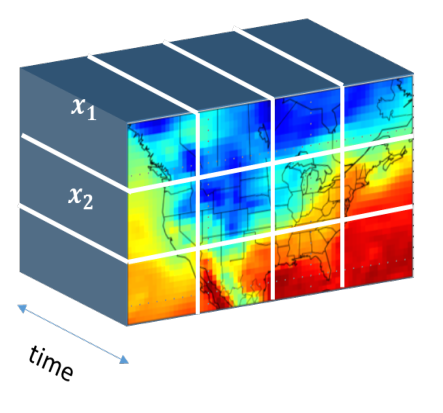
\includegraphics[height=.2\textheight]{Figures/data_cube}
    \caption{The cube represents the global variable $h$ in space and
      time. The sub-cubes specified by the white lines are
      $x_i$. \attn{Can we use $h_i$ here instead of $x_i$?}}
    \label{fig:data_cube}
\end{figure} 


By this definition of $x_i$, the update step for $x_i$ is the
following optimization problem: $x_i^{m+1}:=\argmin_{x_i} ( f_i(x_i) +
(u_i^m)^\top x_i + (\rho/2) \lVert x_i-\tilde{z}_i^m \lVert_2^2)$. We solve this using the PDIP method. As it was explained in \autoref{sec:l1tf_var}, to use PDIP we need to compute the dual problem, which in turn needs the computation of the Fenchel conjugate of the loss function. In addition, referring to \autoref{alg:pdip}, we need to compute the gradient and Jacobian of the conjugate functions. It is important to note that compare to the optimization problem \autoref{eq:l1tf_var}, the loss function in the x-update step in \autoref{eq:ADMM_steps} includes the quadratic term $(\rho/2) \lVert x_i-\tilde{z}_i^m \lVert_2^2$. This makes the computation more involved than \autoref{sec:l1tf_var}. The details of the computations are explained in \autoref{sec:app_consADMM}.\attn{change this to appendix}

\attn{I'm not sure if we want to devote some space to write this as a separate algorithm. The steps are those mentioned in \ref{eq:ADMM_steps} and the x-update is now explained in the appendix. So we may want to remove algorithm \ref{alg:ADMM}. }

The complete ADMM algorithm for estimating the variances is
represented in \autoref{alg:ADMM}. All the computations in the three
updating steps \eqref{eq:ADMM_steps} can be performed in parallel. The
number of rows and columns of the sub-cubes should be chosen so that
the updating of $x_i$ could be performed in one processor. We choose
$3\times3\times521$ sub-cubes. 

\begin{algorithm}[tb]
  \caption{ADMM for sparse estimation of variance of spatio-temporal
    data \attn{Fix this}}
  \label{alg:ADMM}
  \begin{algorithmic}
    \STATE {\bfseries Input:} data $y$, mapping $\mathscr{G}(i,j)$,
    $\rho,\lambda_t,\lambda_s$ 
    \STATE Initialization: $x_i^0=z^0=u_i^0=\textbf{0}$.
    \FOR{$m=1,2,...$ }
    \FOR{$i=1$ {\bfseries to} $N_{sub-cubes}$}
    \STATE compute $\nu_i$ from \eqref{eq:dual_x_update}
    \STATE compute $w_i$ from \eqref{eq:conj_x_update}
    \STATE set $x_i^m:=w_i$
    \ENDFOR
    \STATE Compute $z^m$ from  \eqref{eq:ADMM_steps}
    \STATE Compute $u_i^m$ from  \eqref{eq:ADMM_steps}
    \ENDFOR
  \end{algorithmic}
\end{algorithm}

Because \autoref{alg:ADMM} breaks the large optimization into
sub-problems that can be solved independently, it is amenable to a
split-gather parallelization strategy via, e.g., the map reduce framework.
In each iteration, the
computation time will be equal to the time to solve each sub-problem
plus the time to communicate the solutions on the master processor
and perform the consensus step. Since each sub-problem is
small, with parallelization, the computation time in each iteration
will be small. In addition, our experiments with several values of
$\lambda_t$ and $\lambda_s$ showed that the algorithm converges in few
hundreds iterations. 
\attn{Need to redo this:}Solving each sub-problem on a machine with four
3.20GHz Intel i5-3470 cores takes less than 3 seconds on average, and
so for example if we assume that communication time is 10 seconds and
the algorithm converges in 300 iterations, with parallelization on
$N_{sub-cubes}$ machines, the algorithm will converge in about 1
hour. Assuming that we use $N_{sub-cubes}$ machines and that the
convergence rate of the algorithm is independent of the grid size,
this time will be independent of the grid size. 

If we perform these computations on a single machine, the computation
time grows linearly with $N_{sub-cubes}$. For example, for the data in
a grid over the united states and using $3\times3\times521$ sub-cubes
each iteration of the algorithm will take about 20 minutes on a single
machine and so with 300 iterations it will take several days to
converge. Given that we need to compute the solution for several
values of the parameters $\lambda_t$ and $\lambda_s$, this computation
time is not feasible. 

Therefore, this algorithm is only useful if we can parallelize the
computation over several machines. In the next section, we describe
another algorithm which makes the computation feasible on a single
machine. 

\subsection{Linearized ADMM}
\label{sec:linADMM}

% In this section, we describe \textit{Linearized ADMM algorithm} \citep{parikh_proximal_2014} which, as we will see, makes the computation on a single machine feasible.

\attn{Need a good dummy variable here, it can't be $u$.} Consider the generic optimization problem
$\min_x f(x)+g(Dx)$
where $x\in \mathbb{R}^n$ and $D\in \mathbb{R}^{m\times n}$. Each
iteration of the linearized ADMM
algorithm~\citep{parikh_proximal_2014} for solving this problem 
has the form

\begin{align}
x & \leftarrow \prox_{\mu f} \left(x - (\mu/\rho)D^\top (D x - z + u )\right)\\
z & \leftarrow \prox_{\rho g} \left(z + u\right) \label{eq:linADMM_steps}\\
u & \leftarrow u + D x - z
\end{align}

\noindent where the algorithm parameters $\mu$ and $\rho$ satisfy $0 < \mu < \rho/\norm{D}_2^2$, $z,u\in \mathbb{R}^m$ and the proximal operator is defined as

\begin{equation}
 \prox_{\alpha f}(u) = \min_x \,\, \alpha \cdot f(x)+\frac{1}{2} \norm{ x-u}_2^2.
\label{eq:linADMM_prox}
\end{equation}

\attn{What are $\mu$ and $\rho$?}

\attn{Arash: I explained it above. They are algorithm parameters.}


Clearly, \eqref{eq:l1tf_var_st} has this form necessary for using this algorithm.
% The optimization problem 
% form \eqref{eq:linADMM_opt} by defining
% \begin{align}
% & f(x):= \sum_{k} f_k(x_k) := \sum_{k}x_k+y_{k}^2e^{-x_{k}}\\
% & g(z):= \sum_{l} g_l(z_l) := \sum_{l} \lambda_l |z_l|\label{eq:linADMM_fg}\\
% & z = Dx
% \end{align}
% where $y_k$ is the $k^{th}$ entry of the vector whose entries are
% $y_{ijt}$, and $\lambda_l$ is the $l^{th}$ entry of the vector
% $\Lambda^\top=(\lambda_t\textbf{e}_{n_t}^\top|\lambda_s\textbf{e}_{n_s}^\top)$
% (see \autoref{sec:exten}). 
To perform the steps in \eqref{eq:linADMM_steps}, we need to evaluate
$\prox_{\mu f}$ and $\prox_{\rho g}$. Proximal
algorithms are feasible only if these proximal operators can be
evaluated efficiently which, as we show next, is the case for our
problem.  


\begin{theorem}
  Let $f(h) = \sum_{k} h_{k} + y_{k}^2e^{-h_{k}}$ and $g(x) =
  \norm{x}_1$. Then, 
  \begin{align}
    [\prox_{\mu f}(u)]_k &= \mathscr{W}\bigg(\frac{y_k^2}{\mu}
    \exp\bigg(\frac{1-\mu u_k}{\mu}\bigg) \bigg) + \frac{1-\mu u_k}{\mu},\\
    \prox_{\rho g}(u) &= S_{\rho\lambda}(u)
  \end{align}
where $\mathscr{W}(\cdot)$ is the \textit{Lambert function} \cite{corless_lambertw_1996},  $[S_{\alpha}(u)]_k = \sign(u_k)(|u_k| -\alpha_k)_+$ and
$(v)_+=v\vee 0$.
\end{theorem}
\begin{proof}
  If $f(x)=\sum_k f_k(x_k)$ then $[\prox_{\mu f}(x)]_k =
  \prox_{\mu f_k}(u_k)$. So 
  $[\prox_{\mu f}(u)]_k=\min_{x_k} \,\,
  \mu\big(x_k+y_{k}^2e^{-x_{k}}\big)+\frac{1}{2}  (x_k-u_k)^2.$
  Setting the derivative to 0 and solving for $u_k$ gives the
  result. Similarly, $[\prox_{\rho g}(u)]_\ell=\rho
  \lambda_\ell |z_\ell|+1/2(z_\ell-u_\ell)^2$. This is not differentiable,
  but the solution must satisfy $\rho \cdot \lambda_\ell \cdot \partial
  \big(|z_\ell| \big)=u_\ell-z_\ell$ where $\partial \big(|z_\ell| \big)$ is the
  sub-differential of $|z_\ell|$. The solution is the soft-thresholding
  operator $S_{\rho\lambda_\ell}(u_\ell)$.
\end{proof}

\begin{algorithm}[tb]
  \caption{Linearized ADMM }
  \label{alg:linADMM}
  \begin{algorithmic}
    \STATE {\bfseries Input:} data $y$, penalty matrix $D$,
    $\rho,\lambda_t,\lambda_s >0$.
    \STATE {\bf Set:} $h\leftarrow 0$, $z\leftarrow 0$, $u\leftarrow 0$. 
    \FOR{$m=1,2,...$ }
    \STATE $h_k\leftarrow \mathscr{W}\bigg(\frac{y_k^2}{\mu}
    \exp\bigg(\frac{1-\mu u_k}{\mu}\bigg) \bigg) + \frac{1-\mu u_k}{\mu}$,
    \STATE $z\leftarrow S_{\rho\lambda}(u)$.
    \STATE $u\leftarrow u + Dh-z$
    \ENDFOR
  \end{algorithmic}
\end{algorithm}





\section{Empirical evaluation}
\label{sec:empirical-evaluation}

In this section, we examine both simulated and real spatio-temporal
climate data. All the computations were performed on a Linux machine
with four 3.20GHz Intel i5-3470 cores. 

\subsection{Simulations}
\label{sec:simulations}

\attn{Can we add some type of performance measure? What if we fit 2
  marginal models, spatial only and temporal only. Plus maybe a
  marginal GARCH?}

We generate observations at all time steps and all locations from
independent Gaussian random variables with zero mean. However, the
variance of these random variables follows a smoothly varying function
in time and space

\begin{align}
\sigma^2(t,r,c) & =\sum_{s=1}^{S} W_s(t) \cdot \exp\bigg( \frac{(r-r_s)^2+(c-c_s)^2}{2\sigma_s^2} \bigg); &
W_s(t) & =\alpha_s \cdot t + \exp(\sin(2\pi\omega_s t+\phi_s)) .
\label{eq:sourceVar}
\end{align}

In words, the variance at each time and location is computed as the weighted sum of $S$ bell-shaped functions where the weights are time-varying, consist of a linear trend $\alpha_s \cdot t$ and a periodic term $\beta_s \cdot \sin(2\pi\omega_s t+\phi_s)$. The bell-shaped functions impose the spatial smoothness, and the linear trend and the periodic terms enforce the temporal smoothness similar to the seasonal component in the real climate data. We simulated the data on a 5 by 7 grid and for 780 time steps with $S=4$. The parameters of the variance function are shown in \autoref{tab:sim_params} in Appendix C. For reference, we plot the variance function for all locations at $t=25$ and $t=45$ in as well as the variance across time at $(0,0)$ in \autoref{fig:true_var_spatial} in Appendix C.

We estimated the linearized ADMM for all combinations of values of
$\lambda_t$ and $\lambda_s$ from the sets $\lambda_t \in
\{0,1,5,10,50,100\}$ and $\lambda_s \in \{0,0.05,0.1,0.2,0.3\}$. For
each pair, we then compute the mean absolute error (MAE) between the
estimated variance and the true variance at all locations and all time
steps. For $\lambda_t=5$ and $\lambda_s=0.1$ MAE was minimized. The
left panel of \autoref{fig:true_fitted_var} shows the true and the
estimated standard deviation at location (0,0) using $\lambda_s=0.1$
and $\lambda_t=5$ (blue) and $\lambda_t=100$ (green). As we can see,
larger than optimal value of $\lambda_t$ leads to estimated values
which are ``too smooth".  

\begin{figure}[tb]
  \centering	
  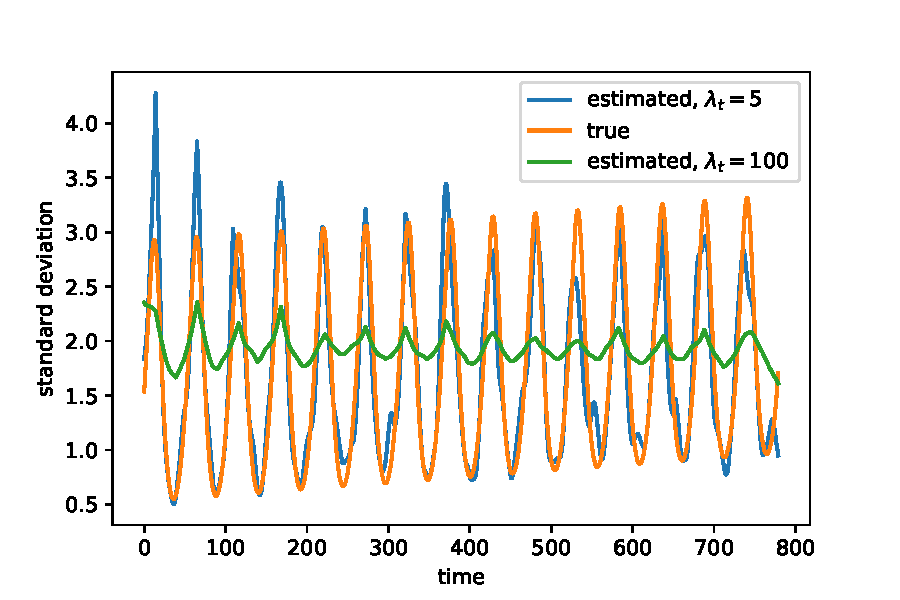
\includegraphics[height=.12\textheight]{Figures/true_fitted_var}
  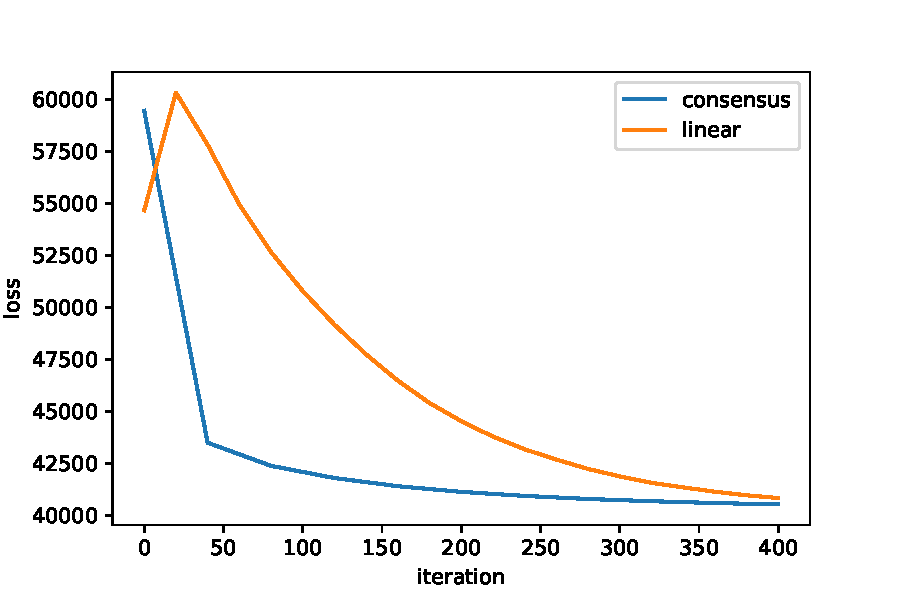
\includegraphics[height=.12\textheight]{Figures/convergence}  
  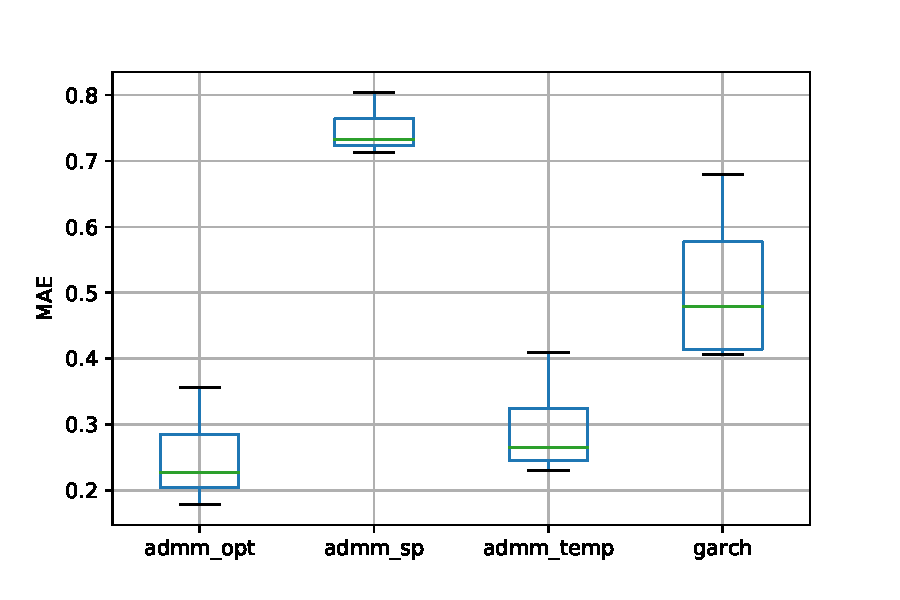
\includegraphics[height=.12\textheight]{Figures/modelComp_MAE}  
  \caption{Left: The true (orange) and estimated standard deviation 
    function at the location (0,0). The estimated values are
    obtained using linearized ADMM with $\lambda_s=0.1$ and two
    values of $\lambda_t$: $\lambda_t=5$ (blue) and
    $\lambda_t=100$ (green). Middle: Convergence speed of linearized and consensus ADMM. Right: MAE for four models: admm\_opt: the proposed model with optimal values of $\lambda_t$ and $\lambda_s$, admm\_temp: no spatial penalty, admm\_sp: no temporal penalty.} \label{fig:true_fitted_var}
\end{figure}

The middle panel of \autoref{fig:true_fitted_var} shows the convergence of Algorithms~\ref{alg:ADMM} and~\ref{alg:linADMM}. Each iteration of the linearized algorithm takes 0.01 seconds on average while each iteration of the consensus ADMM takes about 20 seconds.

To further examine the performance of the proposed model, we next compare it to three models: a model which does not consider the spatial smoothness and so is equivalent to fitting the model in \autoref{sec:l1tf_var} to each time-series separately, a model which does not consider the temporal smoothness, and a GARCH(1,1) model. We simulated 100 datasets using the method explained above with $\sigma_s \sim \mathsf{unif}(4,7)$. The right panel of \autoref{fig:true_fitted_var} shows the boxplot of MAE for these models. Interestingly, the proposed model with optimal parameters outperforms GARCH(1,1) in estimating the true value of the variance.   



\attn{These data are pretty small. Is it possible to do the PDIP?}

\attn{Arash: we can, but why? it will be very slow.}


\subsection{Data analysis}
\label{sec:data}

\autoref{alg:ADMM} is appropriate only if
we parallelize it over multiple machines, and it is significantly
slower on our simulated data, so we do not pursue it
further here. All the results reported in this section are obtained
using \autoref{alg:linADMM}. We
applied this algorithm to the northern hemisphere of the ERA-20C
dataset available from the \href{European Center for Medium-Range
  Weather Forecasts}{https://www.ecmwf.int}. The data are
the 2 meter temperature measured daily at 12 p.m from January 1, 1960
to December 24, 2010. 

In Appendix D, we investigate some properties of the time-series of different locations on earth. We also explain how each time-series is detrended using $\ell_1$-trend filtering method explained in \autoref{sec:ell_1-trend-filt}. \autoref{fig:bloom_estimatedSD} shows a time-series after detrending using this method. The variance of this time-series have a cyclic behavior. The cycles are not regular and their amplitude and frequency change. In addition, the time-series of other locations show different patterns. These observations motivate the need to develop a non-parametric framework for the problem at hand. In this figure, the estimate SD obtained from the method of \autoref{sec:l1tf_var} is also shown. Sine the estimated SD captures the periodic behavior of volatility, it is hard to see the trend in volatility based on these estimated values. Therefore, we compute the annual average of these estimates. However, as this figure shows, the annual trend is not smooth. This is because in the optimization problem \eqref{eq:l1tf_var}, the smoothness of the annual trend is not encouraged. Therefore, in Appendix D we propose a simple method to encourage the smoothness of the annual average trend. The estimated SDs using this method is shown in the right panel of \autoref{fig:bloom_estimatedSD}. The annual average of the estimated SDs shows a linear trend with a positive slope. 

\paragraph{Convergence}

We used the following rule to determine when to stop the optimization: the optimization was stopped if the value of the loss did not improve by at least 0.1\% in 1000 trials. Our experiments showed that the convergence speed depends on the value of $\lambda_t$ and $\lambda_s$. Also, if we use the solution obtained for smaller values of these parameters as the initial value for the larger values (\textit{warm start}), the converges speed improves. 


\paragraph{Model selection}
One common method for choosing the penalty parameters in the Lasso
problems is to find the solution for a range of the values of these
parameters and then choose the values which minimize a model selection
criterion. However, such analyses needs the computation of the degrees
of freedom (df). Several previous work have investigated the df in
generalized lasso problems
\citep{tibshirani_degrees_2012,hu_dual_2015,zeng_geometry_2017}. However,
all these studies have considered the linear regression problem and,
to the best of our knowledge, the problem of computing the df for
generalized lasso with general objective function has not been
considered yet. 

Another approach is to choose the set of values which minimize an
estimate of the expected prediction error obtained by k-fold
cross-validation \citep{tibshirani_regression_1996} . Although this
method is applicable for our problem, it needs k times more
computation. 

In this paper, we use a heuristic method for choosing $\lambda_t$ and
$\lambda_s$: we compute the optimal solution for a range of values of
these parameters and choose the values which minimize
$\mathscr{L}(\lambda_t,\lambda_s)=-l(y|h)+ \sum \lVert D_{total}h
\lVert$. This objective is a compromise between the negative log
likelihood ($-l(y|h)$) and the complexity of the solution ($\sum
\lVert D_{total}h \lVert$). For smoother solutions the value of $\sum
\lVert D_{total}h \lVert$ will be smaller but with the cost of larger
$-l(y|h)$. 

We computed the optimal solution for all the combinations of the
following sets of values: $\lambda_t \in \{0,2,4,8,10,15,200,1000\} \, \, ,
\lambda_s \in \{0,.1,.5,2,5,10\}$. The best combination was $\lambda_t=4$ and $\lambda_s=2$. All the analyses in the next section are performed on the solution for these values. 


\paragraph{Analysis of trend of temperature volatility}

The top row of \autoref{fig:avg_change_estimatedSD} shows the
detrended data, the estimated standard deviation and the yearly
average of these estimates for two cities in the US: Bloomington (left) and San Diego (right). The estimated SD captures the periodic behavior in the variance of the time-series. In addition, the number of linear segments changes adaptively in each time window depending on how fast the variance is changing.  

The yearly average of the estimated SD captures the trend in the
temperature volatility. For example, we can see that in Bloomington,
there is a small positive trend. To determine how the volatility has
changed in each location, we subtract the average of the estimated
variance in 1992 from the average in the following years and compute
their sum. The value of this change in the variance in each location
is depicted in the right panel of \autoref{fig:avg_change_estimatedSD}. The left panel of this figure, shows the average estimated variance in each location. Since the optimal value of the spatial penalty is rather large ($\lambda_s=2$) the estimated variance is spatially very smooth.

It is interesting to note that the trend in volatility is almost zero over the oceans. The most positive trend can be observed in Asia and particularly in south-east Asia.

The bottom panel of \autoref{fig:avg_change_estimatedSD} shows the histogram of change in the estimated SD across the northern hemisphere. As we can see, the SD in most locations on the northern hemisphere had a negative trend in this time period. 

\begin{figure}[tb]
  \centering
  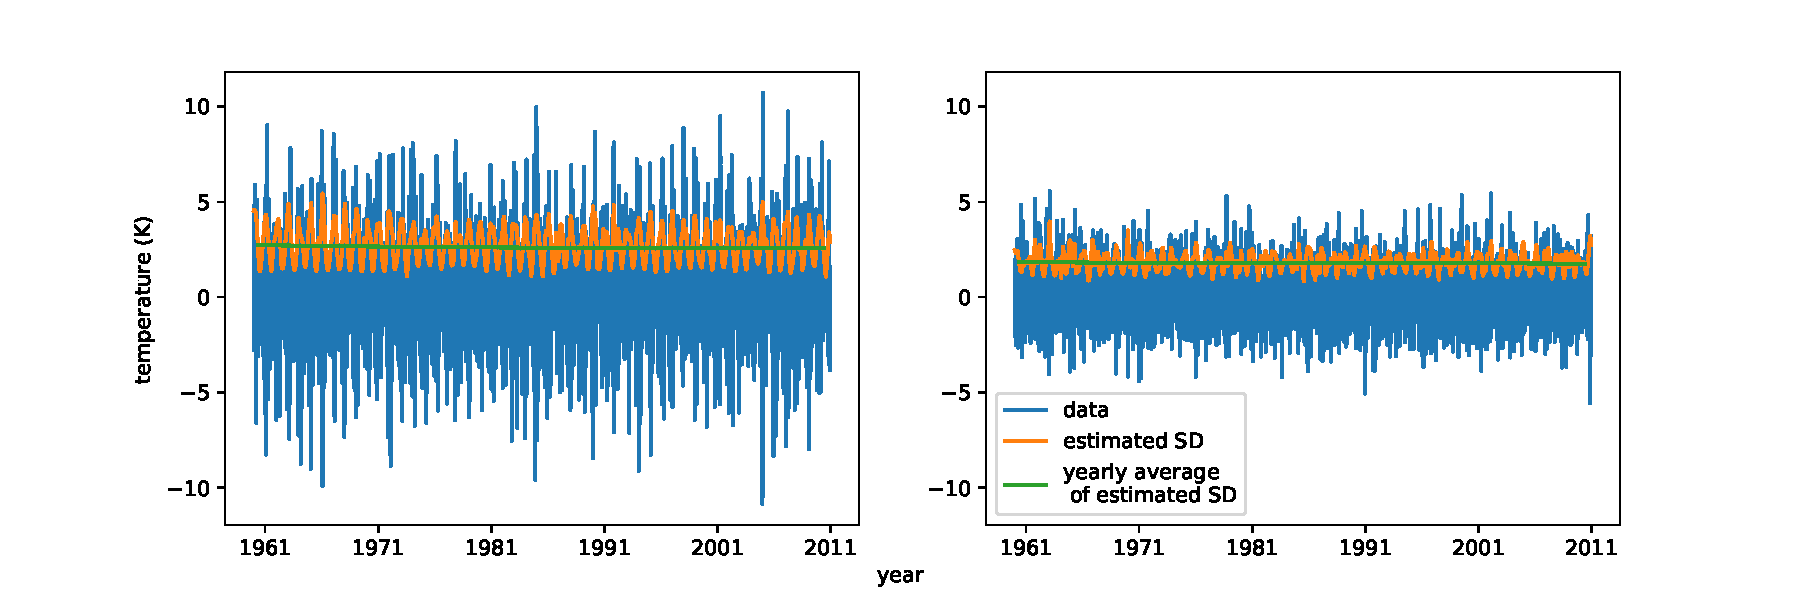
\includegraphics[width=.9 \columnwidth]{Figures/ts_estimatedVar}\\
  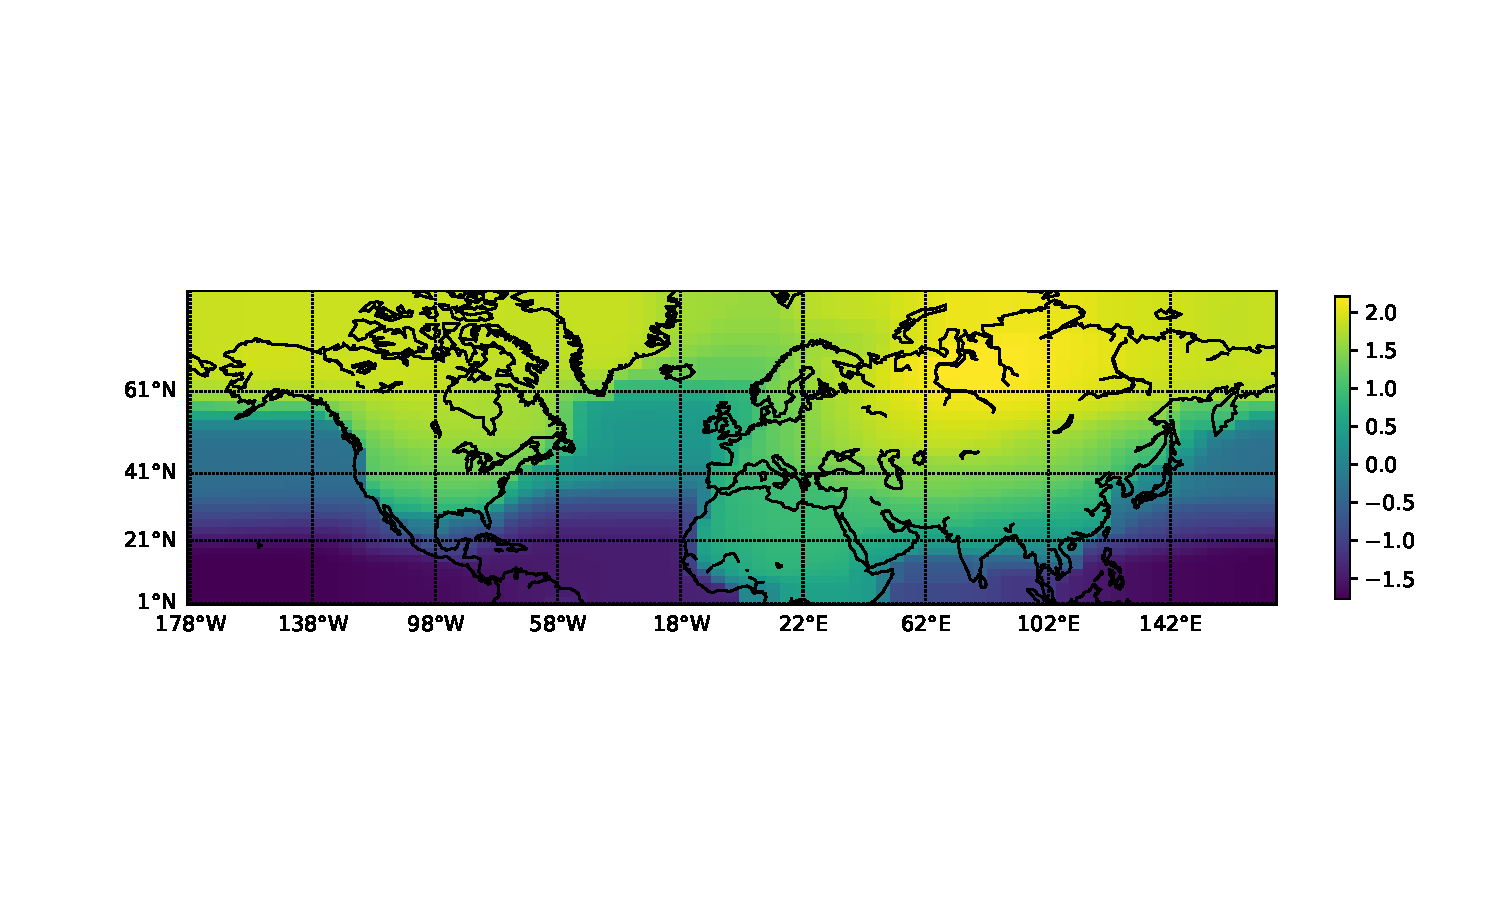
\includegraphics[width=.45\linewidth]{Figures/avg_logVar.pdf}
  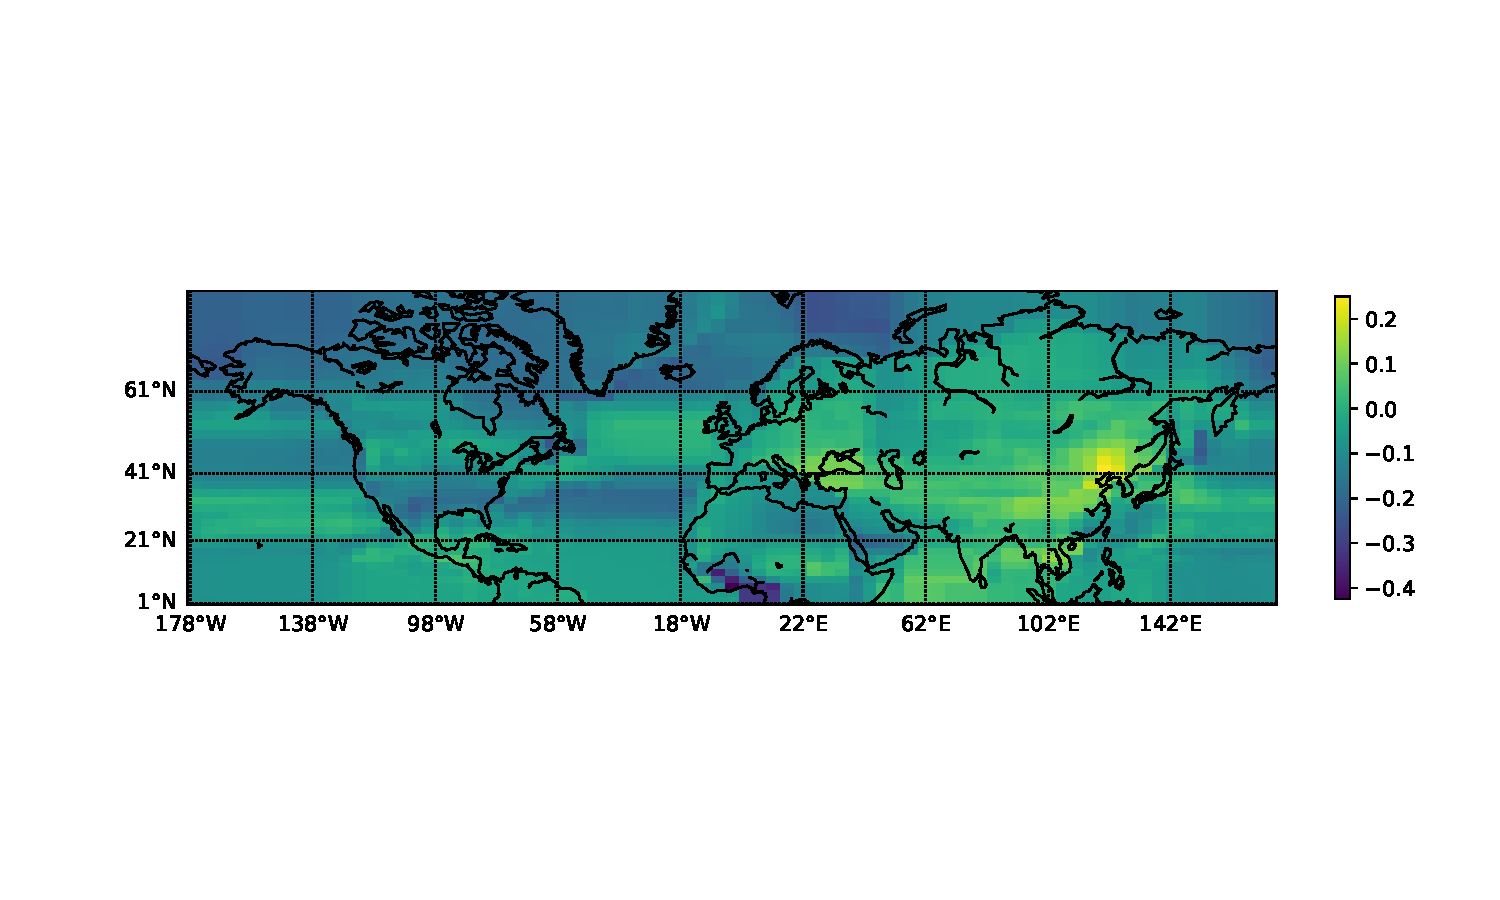
\includegraphics[width=.45\linewidth]{Figures/avg_change_logVar.pdf}\\
    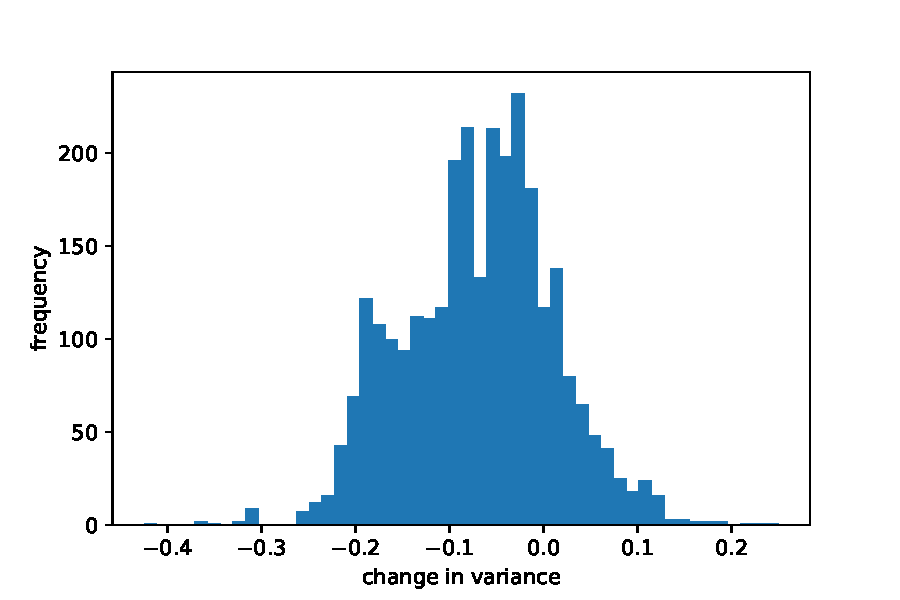
\includegraphics[width=.3\linewidth]{Figures/hist_avg_change.pdf}
  \caption{Top row: Detrended data and the estimated SD for
    Bloomington (left) and San Diego (right). Middle row: the
    average of the estimated variance over the northern hemisphere (left) and the
    change in the variance from 1961 to 2011 (right). Bottom: the histogram of change in estimated SD.} 
  \label{fig:avg_change_estimatedSD}
\end{figure} 

 

\section{Discussion}
In this paper, we proposed a new method for estimating the variance of
spatio-temporal data. The main idea is to cast this problem as a
constrained optimization problem where the constraints enforce smooth
changes in the variance for neighboring points in time and space. In
particular, the solution is piecewise linear in time and piecewise
constant in space. The resulting optimization is in the form of a
generalized LASSO problem with high-dimension, and so applying the
PDIP method directly is infeasible. We therefore developed two
ADMM-based algorithms to solve this problem: the consensus ADMM and
linearized ADMM. 

The consensus ADMM algorithm converges in few hundreds of iterations
but each iteration takes much longer than the linearized ADMM
algorithm. The appealing feature of the consensus ADMM algorithm is
that if it is parallelized on enough number of machines the
computation time per iteration remains constant as the problem size
increases. The linearized ADMM algorithm, on the other hand converges
in few thousands of iterations but each iteration is performed in
split second. However, since the algorithm converges in many
iterations it is not very appropriate for parallelization. The reason
is that after each iteration the solution computed in each machine
should be broadcast to the master machine and this operation takes
some time which depends on the speed of the network connecting the
slave machines to the master. A direction for future research would be
to combine these two algorithms in the following way: the problem
should be split into the sub-problems (as in the consensus ADMM) but
each sub-problem can be solved using linearized ADMM. 

We applied the linearized ADMM algorithm to the surface temperature
data on a grid over the united states, for years 1992-2002. The
results showed that in many locations the variance of the temperature
has increased about 1 unit in 10 years. 

The goal of this paper, however, is not to make any conclusions about
the trend in the variance because we solved the problem only for a
grid over the united states and for 10 years of the data. A thorough
analysis, needs the full solution over the globe and for a longer time
period. The goal of the paper, was to propose the idea of estimating
the trend in variance of spatio-temporal signals using generalized
lasso and to investigate the algorithms for solving the resulting
optimization problem. 

\section{Appendix A}
\label{sec:app_l1tf_var}

In this appendix we provide more details on how to solve the optimization problem \ref{eq:l1tf_var} using PDIP. The objective function is convex but not differentiable. Therefore, to be able to use PDIP we first need to derive the dual of this problem. We note that this is a generalized LASSO problem \citep{tibshirani_solution_2011}. The dual of a generalized LASSO with the objective $f(x)+\lambda \norm{ Dx }_1$ is:  

\begin{align}
\min_\nu&\quad f^*(-D^\top\nu) & \mbox{s.t.}&\quad \norm{ \nu }_\infty \le \lambda
\end{align}

where $f^*(\cdot)$ is the Fenchel conjugate of $f$: $f^*(u)=\max_x u^\top x-f(x)$. It is simple to show that 

\begin{equation}
f^*(u)=\sum_t (u_t-1)\log\frac{y_t^2}{1-u_t} + u_t-1.
\label{eq:conj}
\end{equation}

Each iteration of PDIP involves computing a search direction by taking a Newton step for the system of nonlinear equations $r_w(v,\mu_1,\mu_2)=0$, where $w>0$ is a parameter and

\begin{equation}
  r_w(v,\mu_1,\mu_2):=
	\begin{bmatrix}
	r_{dual}\\
	r_{cent}	
	\end{bmatrix}=
  \begin{bmatrix}
    \nabla f^*(-D^\top v) + \mu_1 - \mu_2\\
    -\mu_1(v-\lambda\one)+\mu_2(v + \lambda\one) -w^{-1}\one
  \end{bmatrix}
\label{eq:resid}
\end{equation}

for $w>0$, where $\mu_1$ and $\mu_2$ are dual variables for the $\ell_\infty$ constraint. Let $A=[\nabla r_{dual}^\top , \nabla r_{cent}^\top]^\top$. The newton step takes the following form

\begin{equation}
r_w(v,\mu_1,\mu_2)+A
\begin{bmatrix}
	\nabla v\\
	\nabla \mu_1\\
	\nabla \mu_2	
	\end{bmatrix}= 0
\label{eq:newton_step}
\end{equation}


We have:

\begin{equation}
A=
\begin{bmatrix}
	\nabla^2 f^*(-D^\top v) & I & -I\\
	-\mathbf{diag(\mu_1)}\one & -v+\lambda\one & \mathbf{0}\\
	\mathbf{diag(\mu_2)}\one & v+\lambda\one & \mathbf{0}
	\end{bmatrix}
\label{eq:delta_r}
\end{equation}

Therefore, to perform the Newton step we need to compute $\nabla f^*(-D^\top v)$ and $\nabla^2 f^*(-D^\top v)$. It is straightforward to show that

\begin{align}
\nabla f^*(-D^\top v) = -\nabla_u f^*(u) D^\top ,\quad u=-D^\top v, \quad (\nabla_u f^*(u))_j=\log\bigg(\frac{y_j^2}{1-u_j}\bigg) \\
\nabla^2 f^*(-D^\top v)=D\nabla_u^2 f^*(u)D^\top, \quad (\nabla_u^2 f^*(u))_j=\mathbf{diag}\bigg(\frac{1}{1-u_j}\bigg)
\end{align}


\section{Appendix B}
\label{sec:app_consADMM}
\attn{put this in nips appendix format}

In this Appendix we give more details on performing the x-update step in \autoref{eq:ADMM_steps}. We need to solve the following optimization problem:

\begin{equation}
\hat{x}:=\argmin_{x} \bigg( \sum_{j=1}^{n_b} (x_j + y_j^2e^{-x_j}) + (\rho/2) \lVert x-\tilde{z} + u \lVert_2^2 + \Lambda^\top |D x| \bigg)
\label{eq:x_update_opt}
\end{equation}

\noindent where $n_b$ is the number of local variables in each sub-cube in \autoref{fig:data_cube}, and for ease of notation we have dropped the subscript $i$ and superscript $m$. Let $f(x)=\sum_{j=1}^{n_b} (x_j + y_j^2e^{-x_j}) + (\rho/2) \lVert x-\tilde{z} + u \lVert_2^2$. As it was explained in \autoref{sec:l1tf_var}, the dual of this optimization problem is: $\min_\nu f^*(-D^\top\nu)$ with the constraints $|\nu_k| \le \Lambda_k$. So to use PDIP we first need to compute the conjugate function $f^*(\cdot)$. We have:


\begin{align}
f^*(\xi) & = \max_x \quad \xi^\top x - f(x)\\
& =  \max_x \quad \sum_{j=1}^{n_b} (\xi_jx_j - x_j - y_j^2e^{-x_j} - (\rho/2)(x_j-\tilde{z}_j+u_j))
\label{eq:conjugate}
\end{align}

Setting the derivative of the terms inside the summation to 0, we obtain:

\begin{equation}
\xi_j-y_j^2e^{-x_j^*}-\rho x_j^* + \rho (\tilde{z}_j-u_j)=0
\label{eq:x_start}
\end{equation}

\noindent where $x^*$ is the maximizer in \ref{eq:conjugate}. Then, it can be shown that $x_j^*$ which satisfies \eqref{eq:x_start} can be obtained as follows:

\begin{align}
x^*_j & = \mathscr{W}\bigg(\frac{y_j^2}{\rho} e^{\phi_j} \bigg) - \phi_j \\
\phi_j & =\frac{1-\xi_j-\rho(\tilde{z}_j-u_j)}{\rho}
\end{align}

In this equation, $\mathscr{W}(\cdot)$ is the \textit{Lambert function} \cite{corless_lambertw_1996}. Finally, the conjugate function is: $f^*(\xi) = \sum_{j=1}^{n_b} (\xi_jx^*_j - x^*_j - y_j^2e^{-x^*_j} - (\rho/2)(x^*_j-\tilde{z}_j+u_j))$.

To use PDIP, we also need to evaluate $\nabla f^*$ and $\nabla^2 f^*$. First note that $\frac{\partial \mathscr{W}(q)}{\partial q} = \frac{\mathscr{W}(q)}{q(1+\mathscr{W}(q))}$ and $\frac{\partial^2 \mathscr{W}(q)}{\partial q^2} = - \frac{\mathscr{W}^2(q)(\mathscr{W}(q)+q)}{q^2(1+\mathscr{W}(q))^3}$. Using the chain rule we get:

%\x^*_j + \xi_j + \frac{\partial \x^*_j}{\partial \xi_j}

\begin{equation}
\frac{\partial f^*(\xi)}{\partial \xi_j}  =  x^*_j  + \frac{\partial x^*_j}{\partial \xi_j} \bigg[ \xi_j -1 + y_j^2 e^{-x_j^*} + \rho (\tilde{z}_j - u_j - x_j^*) \bigg]
\label{eq:d_f*_start}
\end{equation}

\noindent where we have:

\begin{equation}
\frac{\partial x_j^*}{\partial \xi_j} & = \frac{1}{\rho(1+\mathscr{W}((y_j^2/\rho) e^{-\phi_j} ))}
\label{eq:d_x*_start}
\end{equation}

By some tedious but straightforward computation we can obtain the second derivatives:


\begin{align}
\frac{\partial^2 f^*(\xi)}{\partial \xi_j^2} & =  \frac{\partial x_j^*}{\partial \xi_j} - \rho \frac{\partial^2 x_j^*}{\partial \xi_j^2} \bigg[ \phi_j +x_j^* - \tilde{z}_j + u_j \bigg]\\
& \quad + \frac{\partial x_j^*}{\partial \xi_j} \bigg[ 1-y_j^2 \frac{\partial x_j^*}{\partial \xi_j} e^{-x_j^*} -\rho \frac{\partial x_j^*}{\partial \xi_j} \bigg]
\label{eq:d2_f*_start}
\end{align}


\begin{equation}
\frac{\partial^2 x_j^*}{\partial \xi_j^2}  = \frac{\mathscr{W}((y_j^2/\rho) e^{-\phi_j} )}{\rho^2(1+\mathscr{W}((y_j^2/\rho) e^{-\phi_j} ))^3}
\label{eq:d2_x*_start}
\end{equation}

Having computed the conjugate function and its gradient and Jacobian, now we can use a number of convex optimization software packages which have an implementation of PDIP to perform the x-update step inside the ADMM loop. We chose the python API of the \texttt{cvxopt} package ~\citep{andersen_cvxopt:_2013}. 

\section{Appendix C}
Table \autoref{tab:sim_params} lists the parameters used for simulating data in \autoref{sec:simulations}. \autoref{fig:true_var_spatial} shows the variance function obtained from there parameters at $t=25$ (left) and $t=45$ (center).

\begin{table}[tb]
  \caption{Parameters used to simulate data. \attn{Any ideas to take
      up less space with this info?}}
  \label{tab:sim_params}
  \begin{center}
    \begin{tabular}{ccccccc}
      \hline
      $s$ & $r_s$ & $c_s$ & $\sigma_s$ &$\alpha_s$ & $\omega_s$ & $\phi_s$\\
      \hline
      1 & 0 & 0 & 5 & 0.5 & 0.121 & 0 \\
      2 & 0 & 5 & 5 & 0.1 & 0.121 & 0 \\
      3 & 3 & 0 & 5 & -0.5 & 0.121 & $\pi/2$ \\
      4 & 3 & 5 & 5 & -0.1 & 0.121 & $\pi/2$ \\
      \hline
    \end{tabular}
  \end{center}
\end{table} 

\begin{figure}[tb]
  \centering	
  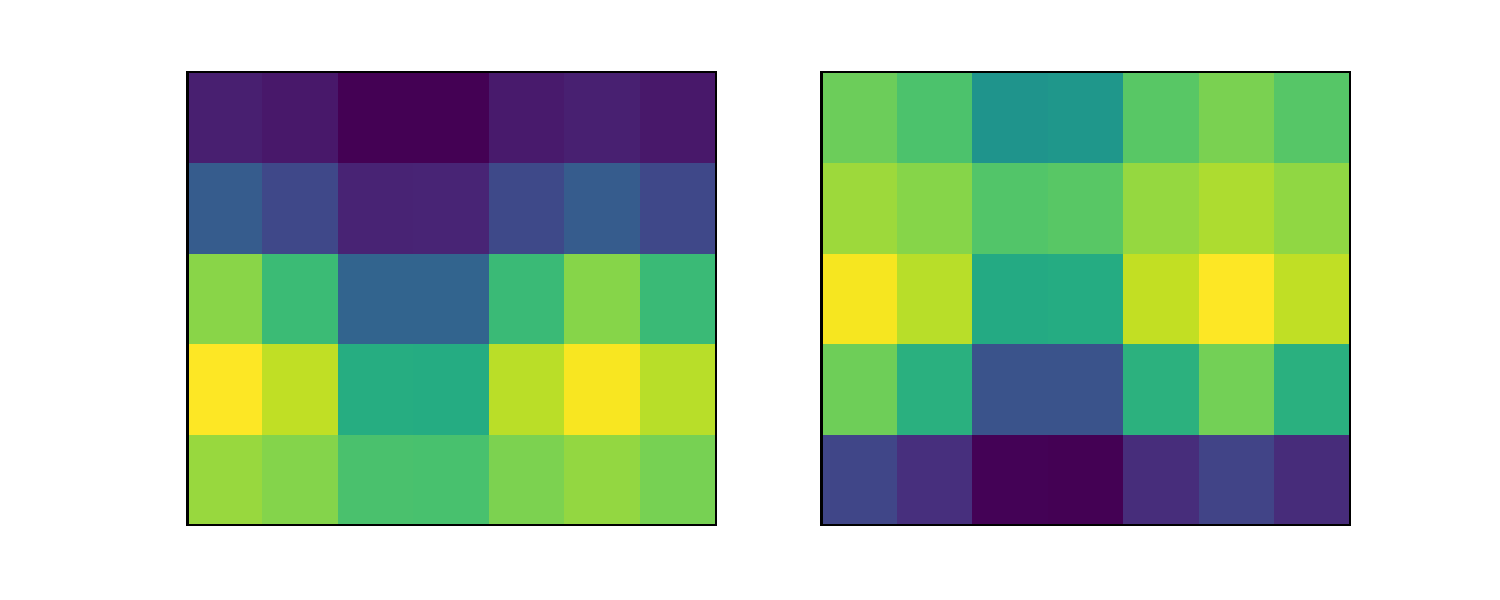
\includegraphics[height=.15\textheight]{Figures/true_var_spatial}
  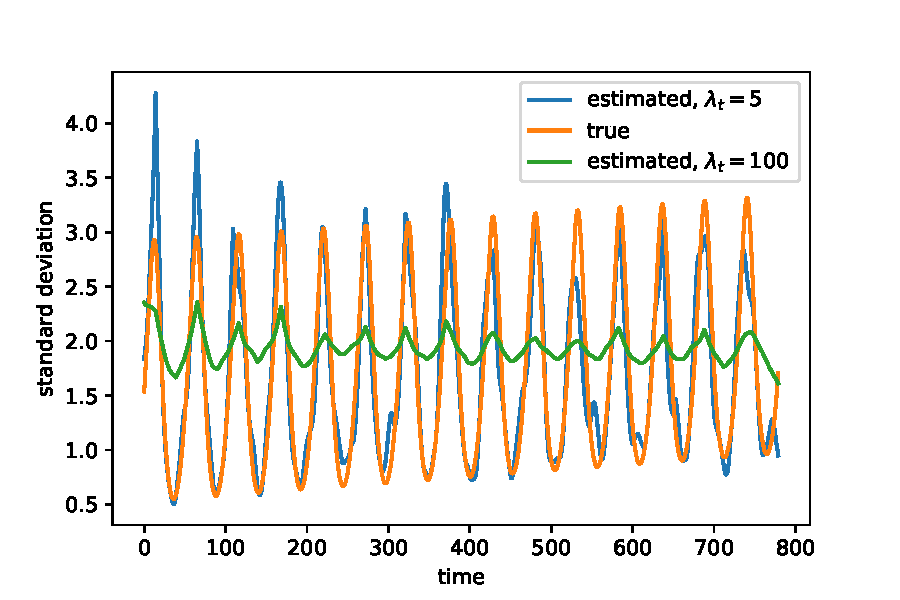
\includegraphics[height=.15\textheight]{Figures/true_fitted_var}
  \caption{Variance function at $t=25$ (left) and $t=45$
    (center). Right: the true (orange) and estimated standard deviation 
    function at the location (0,0). The estimated values are
    obtained using linearized ADMM with $\lambda_s=0.1$ and two
    values of $\lambda_t$: $\lambda_t=5$ (blue) and
    $\lambda_t=100$ (green).} \label{fig:true_var_spatial}
\end{figure}

\section{Appendix D}

In this appendix we examine some of the properties of the time-series of the temperature in ERA-20C dataset. The goal here is to demonstrate some of the difficulties in modeling the trend in the temperature volatility and motivate our methodology.

\autoref{fig:cities_ts} shows the time-series of the temperature of three cities: Bloomington (USA), San Diego (USA) and Manaus (Brazil). The time-series of Bloomington and San Diego show clear cyclic behavior. However, while it seems (qualitatively) that these cycles can be modeled by a sinusoidal function for Bloomington, the same is not true for San Diego. Also, the amplitude of the cycles changes from some years to others. The time-series of Manaus does not show any regular cyclic behavior. This demonstrates the first difficulty in analyzing the variance of this data: to analyze the variance, we first need to remove the cyclic terms from all time-series. However, there is a lot of variations in the cyclic behavior of the time-series of different locations. In addition, some of these cycles cannot be easily modeled by a parametric function \footnote{One might try to model the cycles by the summation of sinusoidal terms with different frequencies. However, for some time-series this may need many terms to be included in the summation to achieve a reasonable level of accuracy. In addition, this model cannot capture the non-stationarity in the cycles.}. To overcome these issues, we use a non-parametric approach to remove the cyclic terms from the time-series and de-trend them. This approach, called \textit{$\ell_1$-trend filtering} is explained in Section 2 of the text. We detrended each time-series separately using this method. For each time-series, we found the optimal value of the penalty parameter using \textit{k-fold cross-validation} with $k=5$. We used the R package \textbf{genlasso} to perform these computations \cite{arnold_efficient_2016}. 

\begin{figure}[tb]
	\centering
	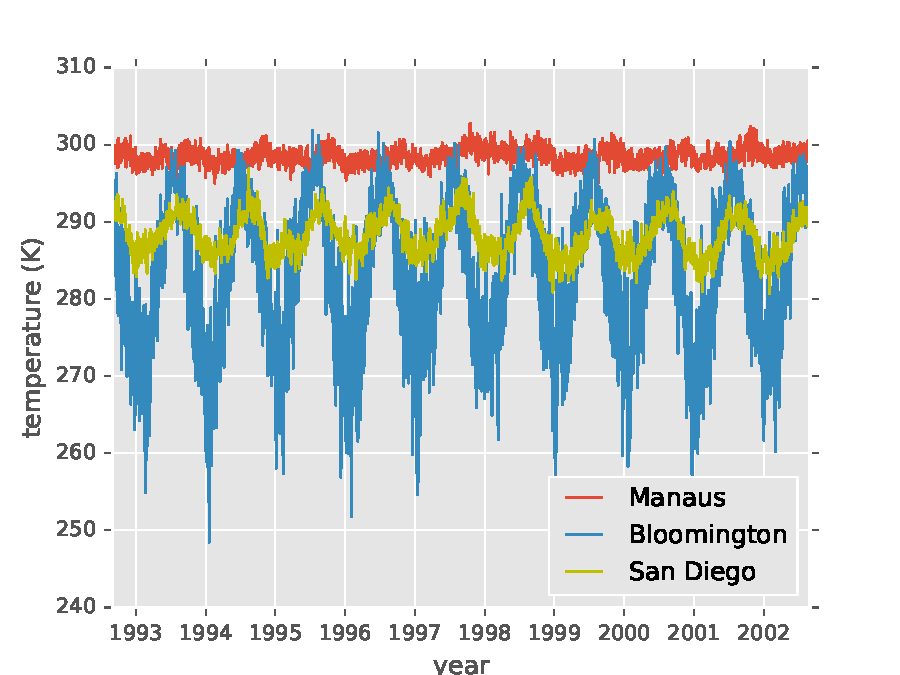
\includegraphics[width=.2\textheight]{Figures/cities_ts}
 	\caption{Time-series of the temperature (in Kelvin) of three cities.}
 	\label{fig:cities_ts}
\end{figure} 

The blue curve in the left panel of \autoref{fig:bloom_estimatedSD} shows the time-series of the temperature of Bloomington after detrending using this method. This figure, reveals another difficulty in estimating the trend of volatility in this data: the variance of this signal, shows cyclic behavior. Also, the cycles are not regular and their amplitude and frequency change. Even if one can describe the behavior of the variance of the time-series at all locations using a single parametric model (for example a variant of the GARCH models \citep{bollerslev_generalized_1986}), it is not clear how the trend in the variance should be investigated in this framework. These observations motivate the need to develop a non-parametric framework for the problem at hand.

\begin{figure}[tb]
  \centering
  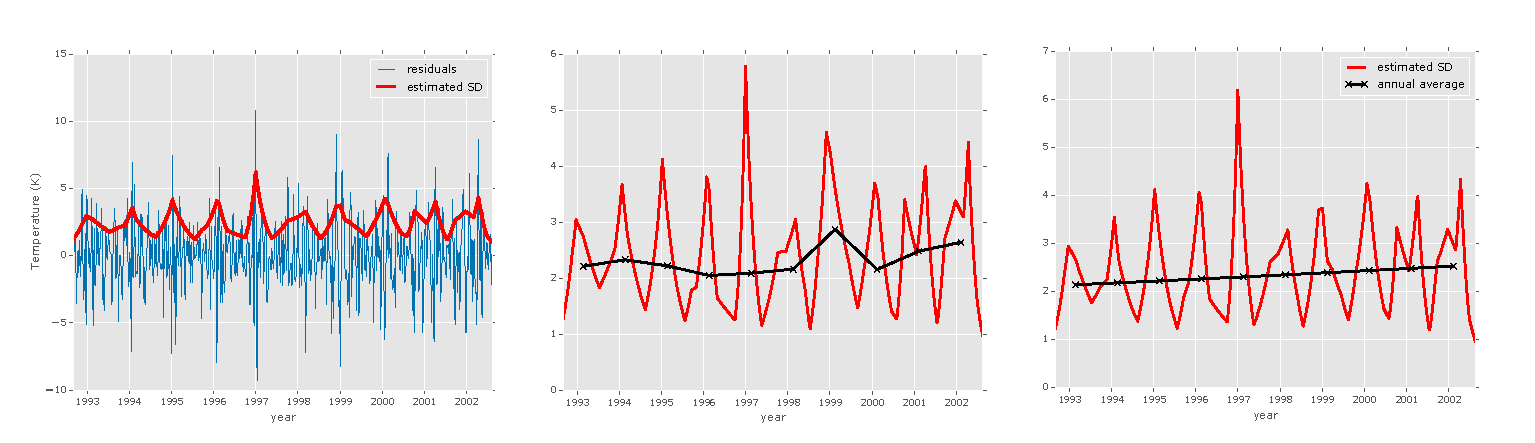
\includegraphics[width=\columnwidth]{Figures/bloom_estimatedSD}
  \caption{Left: The residuals of the time-series of Bloomington
    (averaged weekly) and the estimated SD obtained from the method of
    \autoref{sec:l1tf_var} (red). Middle: the estimated SDs (red) and
    their annual average (black) without imposing the long horizon
    penalty. Right: the same as middle panel but here the long horizon
    penalty is imposed. See the text for more details.} 
  \label{fig:bloom_estimatedSD}
\end{figure} 


The red curve in the left panel of \autoref{fig:bloom_estimatedSD}
shows the estimated SD (which is $\exp(h_t/2)$) of the residuals of
the time-series of Bloomington obtained from out proposed model. To reduce the number of time-steps we work on the weekly averaged of the data. The curve of the estimated SD captures the periodic variations in the
SD of the signal. Just by looking at this curve, it is hard to say if
the SD is decreasing or increasing. Therefore, we compute the average
of the estimated SD for each year. The estimated SD together with this
annual average is shown in the middle panel of
\autoref{fig:bloom_estimatedSD}. As it can be seen, the annual trend
is not smooth. This is because in the optimization problem
\eqref{eq:l1tf_var}, the smoothness of the annual trend is not
encouraged. To remedy this, we add the following long horizon penalty to \eqref{eq:l1tf_var}:
 
\begin{equation}
\sum_{i=1}^{N_{year}-2} \Big\arrowvert \sum_{t=1}^{52} h_{t_1}-2h_{t_2}+h_{t_3}  \Big\arrowvert
\label{eq:lh_penalty}
\end{equation}

where $t_1=52(i-1)+t$, $t_2=52i+t$ and $t_3=52(i+1)+t$. Also, $N_{year}$ is the number of years over which we are performing our analysis (here $N_{year}=10$). Since we are working on the weekly averaged data, each year corresponds to 52 observations. In the matrix form, the penalty \eqref{eq:lh_penalty} adds $N_{year}$ rows to the matrix $D$. The estimated SDs using this penalty matrix is shown in the right panel of \autoref{fig:bloom_estimatedSD}. The annual average of the estimated SDs shows a linear trend with a positive slope.


 

\bibliographystyle{abbrvnat}
\small
\bibliography{nips-references}


\end{document} 

